\documentclass[10pt,landscape]{article}
\usepackage{ctex}
\usepackage{multicol}
\usepackage{calc}
\usepackage{ifthen}
\usepackage[landscape]{geometry}
\usepackage{hyperref}
\usepackage{lipsum}
\usepackage{amsmath}
\usepackage{graphicx}
\usepackage{float}
\usepackage{wrapfig}
\usepackage{xcolor}


% To make this come out properly in landscape mode, do one of the following
% 1.
%  pdflatex latexsheet.tex
%
% 2.
%  latex latexsheet.tex
%  dvips -P pdf  -t landscape latexsheet.dvi
%  ps2pdf latexsheet.ps


% If you're reading this, be prepared for confusion.  Making this was
% a learning experience for me, and it shows.  Much of the placement
% was hacked in; if you make it better, let me know...


% 2008-04
% Changed page margin code to use the geometry package. Also added code for
% conditional page margins, depending on paper size. Thanks to Uwe Ziegenhagen
% for the suggestions.

% 2006-08
% Made changes based on suggestions from Gene Cooperman. <gene at ccs.neu.edu>


% To Do:
% \listoffigures \listoftables
% \setcounter{secnumdepth}{0}


% This sets page margins to .5 inch if using letter paper, and to 1cm
% if using A4 paper. (This probably isn't strictly necessary.)
% If using another size paper, use default 1cm margins.
\ifthenelse{\lengthtest { \paperwidth = 11in}}
	{ \geometry{top=.5in,left=.5in,right=.5in,bottom=.5in} }
	{\ifthenelse{ \lengthtest{ \paperwidth = 297mm}}
		{\geometry{top=1cm,left=1cm,right=1cm,bottom=1cm} }
		{\geometry{top=1cm,left=1cm,right=1cm,bottom=1cm} }
	}

% Turn off header and footer
\pagestyle{empty}
 

% Redefine section commands to use less space
\makeatletter
\renewcommand{\section}{\@startsection{section}{1}{0mm}%
                                {-1ex plus -.5ex minus -.2ex}%
                                {0.5ex plus .2ex}%x
                                {\normalfont\large\bfseries}}
\renewcommand{\subsection}{\@startsection{subsection}{2}{0mm}%
                                {-1explus -.5ex minus -.2ex}%
                                {0.5ex plus .2ex}%
                                {\normalfont\normalsize\bfseries}}
\renewcommand{\subsubsection}{\@startsection{subsubsection}{3}{0mm}%
                                {-1ex plus -.5ex minus -.2ex}%
                                {1ex plus .2ex}%
                                {\normalfont\small\bfseries}}
\makeatother

% Define BibTeX command
\def\BibTeX{{\rm B\kern-.05em{\sc i\kern-.025em b}\kern-.08em
    T\kern-.1667em\lower.7ex\hbox{E}\kern-.125emX}}

% Don't print section numbers
% \setcounter{secnumdepth}{0}


\setlength{\parindent}{0pt}
\setlength{\parskip}{0pt plus 0.5ex}


\newcommand{\dd}{\mathrm{d}}
\newcommand{\pp}{\partial}


% -----------------------------------------------------------------------

\begin{document}

\raggedright
\footnotesize
\begin{multicols}{3}
\section{导论}
\section{燃烧与热化学}
\subsection{概述}
\subsection{热力学参数关系式回顾}
\subsubsection{广延量和强度量}
\textbf{广延量:}取决于物质的数量(质量或物质的量),一般大写;{\textbf{强度量:}单位质量(或物质的量)来表示},数值与物质的量无关。\textit{单位物质的量的在本书中会加上划线},如$\overline{u}$,单位质量的则不加划线,如$u$。

\subsubsection{状态方程}
\begin{eqnarray}
    PV&=&nR_uT\\
    PV&=&mRT\\
    Pv&=&RT\\
    P&=&\rho RT
\end{eqnarray}
$R_u=8315~\mathrm{J/(kmol\cdot K)}$, $R=R_u/\mathrm{MW}$, $\rho=1/v=m/V$.

\subsubsection{状态热方程}

\begin{eqnarray}
    u&=&u(T,v)\\
    h&=&h(T, P)
\end{eqnarray}

\begin{eqnarray}
    \mathrm{d}u&=&\left({\frac{\partial u}{\partial T}}\right)_{v}\mathrm{d}T+\left({\frac{\partial u}{\partial v}}\right)_{T}\mathrm{d}v\\ 
    \mathrm{d}h&=&\left({\frac{\partial h}{\partial T}}\right)_{p}\mathrm{d}T+\left({\frac{\partial h}{\partial P}}\right)_{T}\mathrm{d}P
\end{eqnarray}


\begin{eqnarray}
    c_{v}&\equiv&\left(\frac{\partial u}{\partial T}\right)_{v}\\
c_{p}&\equiv&\left({\frac{\partial h}{\partial T}}\right)_{P}
\end{eqnarray}

对于理想气体,$(\partial u/\partial v)_T$和$(\partial h/\partial P)_{T}$都为0。所以理想气体的状态热方程为:
\begin{eqnarray}
    u(T)-u_{\mathrm{ref}}&=&\int_{T_{\mathrm{ref}}}^{T}c_{v}\,\mathrm{d}T\\ 
    h(T)-h_{\mathrm{ref}}&=&\int_{T_{\mathrm{ref}}}^{T}c_{p}\,\mathrm{d}T.
\end{eqnarray}

\subsubsection{理想气体混合物}
组份$i$的摩尔分数$\chi_i$:
\begin{equation}
    \chi_{i}\equiv\frac{N_{i}}{N_{1}+N_{2}+\cdots+N_{i}+\cdots}=\frac{N_{i}}{N_{\mathrm{tot}}}
\end{equation}
组份$i$的质量分数$Y_i$:
\begin{equation}
    Y_{i}\equiv\frac{m_{i}}{m_{1}+m_{2}+\cdots+m_{i}+\cdots}=\frac{m_{i}}{m_{\mathrm{tot}}}
\end{equation}
他们之间存在着如下的换算关系:
\begin{equation}
    Y_{i}=\chi_{i}\mathrm{M}\mathrm{W}_{i}/\mathrm{M}\mathrm{W}_{\mathrm{mix}}
\end{equation}
\begin{equation}
    \chi_{i}=Y_{i}\mathrm{MW}_{\mathrm{mix}}/\mathrm{MW}
\end{equation}
对于混合物的摩尔质量:
\begin{equation}
    \mathrm{MW}_\mathrm{mix} = \sum_i \chi_i \mathrm{MW}_i
\end{equation}
\begin{equation}
    \mathrm{MW}_\mathrm{mix} = \frac{1}{\sum_i (Y_i/\mathrm{MW}_i)}
\end{equation}

混合物的强度量可以用各物质的强度量加权计算得到,对于组份的熵,我们有:
\begin{equation}
    s_{i}(T,P_{i})=s_{i}(T,P_{\mathrm{ref}})-R\ln{\frac{P_{i}}{P_{\mathrm{ref}}}}
\end{equation}
\begin{equation}
    \bar{s}_{i}(T,P)=\bar{s}_{i}(T,P_{\mathrm{ref}})-R_{u}\ln{\frac{P_{i}}{P_{\mathrm{ref}}}}\,.
\end{equation}

\subsubsection{蒸发潜热}
aka 蒸发焓,
\begin{equation}
    h_{fg}(T,P)\equiv h_{\mathrm{vapor}}(T,P)-h_{\mathrm{liquid}}(T,P),
\end{equation}

给定温度和压力计算蒸发潜热的方法,Clausius-Claperon方程,
\begin{equation}
    \frac{\mathrm{d}P_{\mathrm{sat}}}{P_{\mathrm{sat}}}=\frac{h_{f g}}{R}\,\frac{\mathrm{d}T_{\mathrm{sat}}}{T_{\mathrm{sat}}^{2}}.
\end{equation}

\subsection{热力学第一定律}
\subsubsection{第一定律——定质量}
\subsubsection{第一定律——控制体}

\subsection{反应物和生成物的混合物}
\subsubsection{化学计量学}
对于碳氢燃料C$_x$H$_y$,
\begin{equation}
    \begin{aligned}
        &C_x\mathrm{H}_y + a(\mathrm{O}_2 + 3.76\mathrm{N}_2)\rightarrow\\
        & x\mathrm{CO}_2 + \frac{y}{2}\mathrm{H}_2\mathrm{O} + 3.76a\mathrm{N}_2
    \end{aligned}
\end{equation}



其中,
$$
a=x+y/4.
$$
\textbf{化学当量的空-燃比}:
\begin{equation}
    (A/F)_{\mathrm{stolc}}=\left(\frac{m_{\mathrm{air}}}{m_{\mathrm{fuel}}}\right)_{\mathrm{stoic}}=\frac{4.76a}{1}\frac{M W_{\mathrm{air}}}{MW_{\mathrm{fuel}}},
\end{equation}
\textbf{当量比}:
\begin{equation}
    \Phi={\frac{(A/F)_{\mathrm{stoic}}}{(A/F)}}={\frac{(F/A)}{(F/A)_{\mathrm{stoic}}}}
\end{equation}
当量空气百分比=100\%/$\Phi$,过量空气百分比=(1-$\Phi$)/$\Phi\times$100\%

\subsubsection{绝对(或标准)焓和生成焓}

绝对焓=标准生成焓+显焓的变化,

\begin{equation}
    \overline{h}_i(T) = \overline{h}_{f,i}^0(T_\mathrm{ref})+\Delta\overline{h}_{s,i}(T),
\end{equation}

\textbf{参考温度:}$T_\mathrm{ref}=25^\circ \mathrm{C}$(298.15 K),\textbf{参考压力:}$P_\mathrm{ref}=$1atm(101 325 Pa)。

对于标准生成焓:元素最自然状态时的生成焓为0,比如氧气,氮气等。

\subsubsection{燃烧焓和热值}
\textbf{燃烧焓}定义为(反应物和产物\textit{都处于标准状态下}):
\begin{equation}
    \Delta h_{R}\equiv q_{c v}=h_{\mathrm{prod}}-h_{\mathrm{reac}},
\end{equation}
\textbf{燃烧热}$\Delta h_c$(也称为热值)为燃烧焓的相反数。
\begin{itemize}
    \item \textbf{高位热值}(HHV):假设所有的产物都凝结成液化水时的燃烧热。
    \item \textbf{地位热值}(LHV):没有水凝结成液态的情况下的燃烧热。
\end{itemize}

\subsection{绝热燃烧温度}

\textbf{定压绝热燃烧温度: }
\begin{equation}
    h_{\mathrm{reac}}(T_{i},P)=h_{\mathrm{prod}}(T_{a d},P).
\end{equation}

\begin{figure}[H]
    \centering
    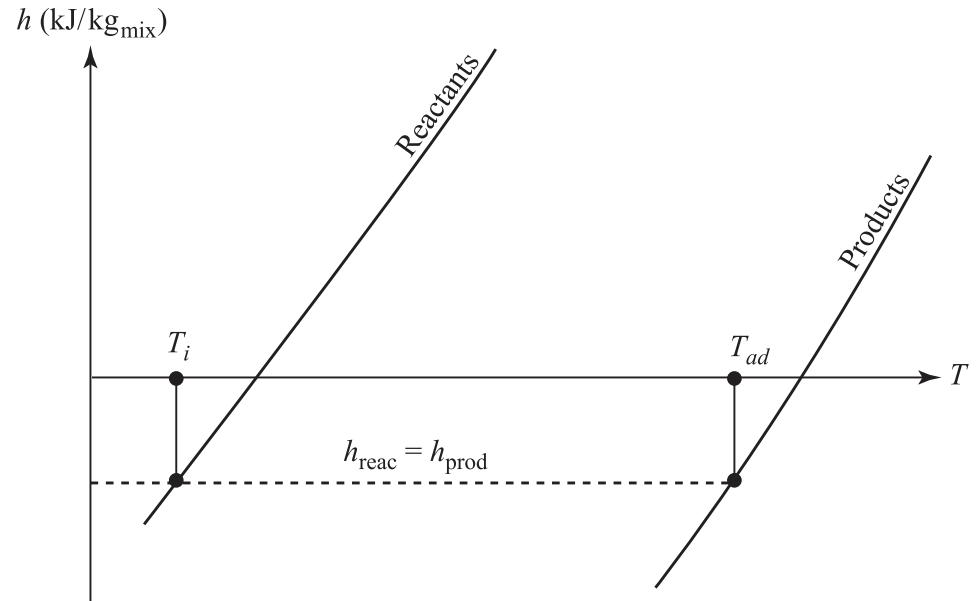
\includegraphics[width=.23\textwidth]{img/ad_T.png}
\end{figure}

\textbf{定容绝热燃烧温度:}反应前后内能相等,
\begin{equation}
    U_{\mathrm{reac}}(T_{\mathrm{init}},P_{\mathrm{init}})=U_{\mathrm{prod}}(T_{a d},P_{f}),
\end{equation}

写成焓的形式:
\begin{equation}
    \begin{aligned}
        H_{\mathrm{reac}}-H_{\mathrm{prod}}-V(P_{\mathrm{init}}-P_{f})&=0.\\
        H_{\mathrm{reac}}-H_{\mathrm{prod}}-R_{u}(N_{\mathrm{reac}}T_{\mathrm{init}}-N_{\mathrm{prod}}T_{a d})&=0.
    \end{aligned}
\end{equation}

\subsection{化学平衡}
\subsubsection{第二定律的讨论}

单个组份的熵计算公式:
\begin{equation}
    \overline{{{s}}}_{i}=\overline{{{s}}}_{i}^{0}(T_{\mathrm{ref}})+\int_{T_{\mathrm{ef}}}^{T_{f}}\overline{{{c}}}_{p,i}\,\frac{\mathrm{d}T}{T}-R_{u}\,\ln\frac{P_{i}}{P^{0}},
\end{equation}

对于封闭系统,反应自发发生的条件为$\mathrm{d}S\ge 0$。平衡条件为:$(\mathrm{d}S)_{U,V,m}=0$。

\subsubsection{吉布斯函数}

单个组份的吉布斯函数的计算:

\begin{equation}
    \overline{{{g}}}_{i,T}=\overline{{{g}}}_{i,T}^{o}+R_{u}T\ln\left(P_{i}/P^{o}\right)
\end{equation}

对于开口系统,我们采用吉布斯函数,它的定义为 $G\equiv H-TS$。这是第二定律表示为$(\mathrm{d}G)_{T,P,m}\le 0$的形式。在平衡时,开口系统的第二定律可以写作$(\mathrm{d}G)_{T,P,m}=0$。

{
    \scriptsize\color{gray}
    考虑广延量,理想气体的吉布斯方程为:
    \[
        G_{\mathrm{mix}}=\sum N_{i}\overline{{{g}}}_{i,T}=\sum N_{i}\bigl[\bar{g}_{i,T}^{0}+R_{u}T\ln\bigl(P_{i}/P^{0}\bigr)\bigr]
    \]
    对上面的式子取微分,得到平衡条件,可以写作:
    \[
        \begin{aligned}
        &\sum{\mathrm{d}{N}}_{i}\left[\bar{g}_{i,T}^{0}+R_{u}T\ln\left(P_{i}/P^{0}\right)\right]+\\
        &\sum{N}_{i}\mathrm{d}\left[\bar{g}_{i,T}^{0}+R_{u}T\ln\left(P_{i}/P^{0}\right)\right]=0.
        \end{aligned}
    \]
    考虑到总压不变,也就是分压变化的和不变,因此式子中的第二项等于零,它可以被简化为:
    \[\sum{\mathrm{d}{N}}_{i}\left[\bar{g}_{i,T}^{o}+R_{u}T\ln\left(P_{i}/P^{0}\right)\right]=0\]
    对于一个一般的系统,我们将化学反应写作
    \[a\mathbf{A}+b\mathbf{B}+\cdots\leftrightarrow e\mathbf{E}+f\mathbf{F}+\cdots\]
    由于物质的摩尔数变化和化学计量数成正比,因此我们可以将平衡表达式展开写作:
    \[
        \begin{aligned}
            &-a\Bigl[\bar{g}_\mathrm{A,T}^{o}+R_{u}T\ln\bigl(P_{\mathrm{A}}/P^{o}\bigr)\Bigr]\\
            &-b\Bigl[\bar{g}_{\mathrm{B,T}}^{o}+R_{u}T\ln\bigl(P_{\mathrm{B}}/P^{o}\bigr)\Bigr]-\cdots\\
            &+e\Bigl[\overline{{{g}}}_{\scriptscriptstyle\mathrm{E,}T}^{o}+R_{u}T\ln\bigl(P_{\scriptscriptstyle\mathrm{E}}/P^{o}\bigr)\Bigr]\\
            &+f\Bigl[\overline{{{g}}}_{\scriptscriptstyle\mathrm{F,}T}^{o}+R_{u}T\ln\bigl(P_{\scriptscriptstyle\mathrm{F}}/P^{o}\bigr)\Bigr]+\cdots=0.
        \end{aligned}
    \]
    合并整理一下不难得到:
    \[
        \begin{aligned}
            &-\Bigl(e\bar{g}_{\mathrm{E},T}^{o}+f\overline{{{g}}}_{\mathrm{F},T}^{o}+\cdot\cdot\cdot-a\overline{{{g}}}_{\mathrm{A},T}^{o}-b\overline{{{g}}}_{\mathrm{B},T}^{o}-\cdots\Bigr)\\
            &=R_{u}T\ln{\frac{\left(P_{\mathrm{E}}/P^{o}\right)^{e}\cdot\left(P_{\mathrm{F}}/P^{o}\right)^{f}\cdot\mathrm{etc.}}{\left(P_{\mathrm{A}}/P^{o}\right)^{a}\cdot\left(P_{\mathrm{B}}/P^{o}\right)^{b}\cdot\mathrm{etc.}}}
        \end{aligned}\]
}
我们定义\textbf{标准状态吉布斯函数差 $\Delta G_T^0$}为:
\begin{equation}
    \Delta G_T^0 = (e\bar{g}_{\mathrm{E},T}^{o}+f\overline{{{g}}}_{\mathrm{F},T}^{o}+\cdot\cdot\cdot-a\overline{{{g}}}_{\mathrm{A},T}^{o}-b\overline{{{g}}}_{\mathrm{B},T}^{o}-\cdots)
\end{equation}
\textbf{平衡常数 \(K_p\)}为:
\begin{equation}
    K_{p}={\frac{\left(P_{\mathrm{E}}/P^{o}\right)^{e}\cdot\left(P_{\mathrm{F}}/P^{o}\right)^{f}\cdot\mathrm{etc.}}{\left(P_{\mathrm{A}}/P^{o}\right)^{a}\cdot\left(P_{\mathrm{B}}/P^{o}\right)^{b}\cdot\mathrm{etc.}}}.
\end{equation}
这时,定压,定温条件下的化学平衡表达式就可以被写作:
\begin{equation}
    \Delta G_T^0 = -R_u T\ln K_p
\end{equation}
\begin{itemize}
    \item 如果\(\Delta G_T^0\)大于零,那么\(K_p\)小于1,反应向左进行(偏向反应物、几乎不反应)。
    \item 如果\(\Delta G_T^0\)小于零,那么\(K_p\)大于1,反应向右进行(偏向产物,趋于完全反应)。
\end{itemize}

{
    \scriptsize
    如果将\(\Delta G_T^0\)写作:
    \[
        \Delta G_T^0 = \Delta H^0 - T\Delta S^0
    \]
    的形式,平衡常数可以被写作:
    \[
        K_p = \mathrm{e}^{-\Delta H^0/R_u T}\cdot \mathrm{e}^{\Delta S^0/R_u}
    \]
    不难发现,
    \begin{itemize}
        \item 当反应的焓变小于零,反应放热,系统能量降低;
        \item 熵变大于零。
    \end{itemize}都会导致反应偏向于产物,\(K_p>1\)。
}

\subsubsection{复杂系统}

\subsection{燃烧的平衡产物}
\subsubsection{全平衡}
考虑实际的燃烧过程,最大燃烧温度一般发生在略微富燃料当量比的状态(\(\Phi\approx 1.05)\)。

\section{传质引论}
\subsection{概述}
\subsection{传质入门}
\subsubsection{传质速率定律}
\begin{itemize}
    \item 菲克扩散定律
    对于一维双组份扩散的情况:
    \begin{equation}\label{equ:fick_law_1d}
        \dot{m}_A'' = Y_A(\dot{m}_A'' + \dot{m}_B'') - \rho \mathcal{D}_\mathrm{AB}\frac{\dd Y_A}{\dd x}
    \end{equation}{\tiny 这里要特别注意,虽然\(\dot{m}_A'' + \dot{m}_B''=\dot{m}''\),但并不意味者\(Y_A \dot{m}''\)就等于\(\dot{m}_A''\)。因为当中还涉及到了扩散作用。}

    \textbf{质量通量}的定义为垂直于流动方向的单位面积质量流量:
    \begin{equation}
        \dot{m}_A'' = \dot{m}_A/A.
    \end{equation}

    可以写成更一般的形式:

    \begin{equation}
        \dot{m}_{\mathrm{A}}^{\prime\prime}=Y_{\mathrm{A}}\,(\dot{m}_{\mathrm{A}}^{\prime\prime}+\dot{m}_{\mathrm{B}}^{\prime\prime})-\rho D_{\mathrm{AB}}\nabla Y_{\mathrm{A}},
    \end{equation}
    \begin{equation}
        \dot{N}_{\mathrm{A}}^{\prime\prime}=\chi_{\mathrm{A}}(\dot{N}_{\mathrm{A}}^{\prime\prime}+\dot{N}_{\mathrm{B}}^{\prime\prime})-c D_{\mathrm{AB}}{\nabla}\chi_{\mathrm{A}},
    \end{equation}
    
    其中\(c\)是混合物的浓度(kmol/m\(^3\))。

    如果我们同时考虑A和B的扩散,将两个物质的式~\ref{equ:fick_law_1d}相加,可以得到:

    \begin{equation}
        -\rho\mathcal{D}_\mathrm{AB}\frac{\dd Y_A}{\dd x} - \rho\mathcal{D}_\mathrm{BA}\frac{\dd Y_B}{\dd x} = 0
    \end{equation}

    \item 扩散的分子基础
    扩散系数和温度及压强的关系:
    \begin{equation}
        \mathcal{D}_\mathrm{AB} \propto T^{3/2}P^{-1}
    \end{equation}

    而质量通量实质上是和\(\rho \mathcal{D}_\mathrm{AB}\)相关,它仅和温度相关:
    \begin{equation}
        \rho\mathcal{D}_\mathrm{AB}\propto T^{1/2}
    \end{equation}
    \item 与热传导的比较
\end{itemize}

\subsubsection{组分守恒}
考虑化学反应:
\begin{equation}
    \frac{\dd m_{\mathrm{A}, cv}}{\dd t} = [\dot{m}_A'' A]_x - [\dot{m}_A'' A]_{x+\Delta x} + \dot{m}_A''' V
\end{equation}

经过整理可以得到:
\begin{equation}
    \frac{\pp(\rho Y_A)}{\pp t} = -\frac{\pp}{\pp x}\left[Y_A\dot{m}'' - \rho \mathcal{D}_\mathrm{AB}\frac{\pp Y_A}{\pp x}\right] + \dot{m}_A'''
\end{equation}

对于稳态的情况:
\begin{equation}
    \dot{m}_A''' - \frac{\dd}{\dd x}\left[Y_A\dot{m}'' - \rho\mathcal{D}_\mathrm{AB}\frac{\dd Y_A}{\dd x}\right] = 0.
\end{equation}

把括号里面的东西打包的话其实也可以写作:
\begin{equation}
    \dot{m}_A''' - \nabla\cdot \dot{m}_A'' = 0
\end{equation}

\subsection{传质的应用实例}
\subsubsection{斯蒂芬问题}

\begin{wrapfigure}{l}{.15\textwidth}
    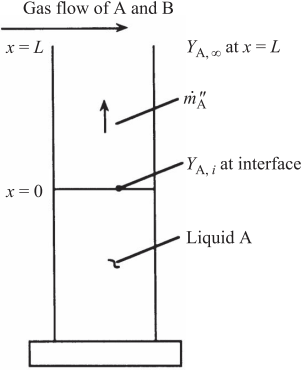
\includegraphics[width=.15\textwidth]{img/stefan.png}
\end{wrapfigure}

我们考虑液体A在玻璃圆通内保持一个固定的高度,假设B在A中不可溶解,由此圆柱中存在着一个B的滞止层。对于这个问题,A的质量通量为:

\begin{equation}\tiny
    \dot{m}''_A = \frac{\rho \mathcal{D}_\mathrm{AB}}{L}\ln\left(\frac{1-Y_{A,\infty}}{1-Y_{A,i}}\right)
\end{equation}

推导过程如下:
{\scriptsize\color{gray}

由于B的量通量为0,基于菲克定律式~\ref{equ:fick_law_1d},我们可以写出
\[
    \dot{m}_A'' = Y_A\dot{m}_A'' - \rho \mathcal{D}_\mathrm{AB}\frac{\dd Y_A}{\dd x}
\]对之整理并分离变量:
\[
    -{\frac{\dot{m}_{\mathrm{A}}^{\prime\prime}}{\rho D_{\mathrm{AB}}}}\mathrm{d}x={\frac{\mathrm{d}Y_{\mathrm{A}}}{1-Y_{\mathrm{A}}}}.
\]
积分解得:
\[
    -{\frac{\bar{m}_{\mathrm{A}}^{\prime\prime}}{\rho D_{\mathrm{AB}}}}\,x=-\ln[1-Y_{\mathrm{A}}]+C,
\]结合已知边界条件,\(Y_A(x=0)=Y_{A,i}, Y_A(x=L)=Y_{A,\infty}\)。}

就可以写出质量分数的计算公式:

\begin{equation}
    Y_A(x) = 1 - (1-Y_{A,i})\exp\left(\frac{\dot{m}_A'' x}{\rho\mathcal{D}_\mathrm{AB}}\right)
\end{equation}

\subsubsection{液-气界面的边界条件}

不难写出\(\chi_{A,i} = P_\mathrm{sat}/P\),由此可以确定质量分数应该为:
\begin{equation}
    Y_{A,i} = \frac{P_\mathrm{sat}(T_\mathrm{liq, i})}{P}\frac{\mathrm{MW}}{\mathrm{MW}_\mathrm{mix, i}}
\end{equation}

认为液-气界面上维持温度的连续性,那么:
\[
    T_\mathrm{liq,i}(x=0^-) = T_\mathrm{vap, i}(x=0^+) = T(0)
\]


\subsubsection{液滴蒸发}

\textbf{假设}:
{\scriptsize
    \begin{enumerate}
        \item 蒸发过程是准稳态的。
        \item 液滴的温度均一,进而假设温度为低于液体的沸点的某一定值。
        \item 液滴表面蒸气的质量分数由液滴温度下的液体-蒸气平衡确定。
        \item 假设所有的热物理参数——特别是\(\rho\mathcal{D}\)——是常数。
    \end{enumerate}
}

\textbf{蒸发速率}:

从某种意义上说,这里的液滴蒸发问题其实就是一个加强版的球状的斯蒂芬流。定义\textbf{传质数}\(B_Y\)为:
\begin{equation}
    B_Y = \frac{Y_{A,s}-Y_{A,\infty}}{1 - Y_{A,s}}
\end{equation}
蒸发速率可以被写作:
\begin{equation}\label{equ:evo_rate}
    \dot{m}_A''' = {4\pi r_s \rho \mathcal{D}_\mathrm{AB}}\ln({1+B_Y})
\end{equation}

具体的推倒过程如下所示:

{
    \scriptsize\color{gray}
    首先,液滴的蒸发速率可以被写作
    \[
        \dot{m}(r) = 4\pi r^2 \dot{m}''
    \]
    将之带入到菲克定律~\ref{equ:fick_law_1d}的表达式中,并且认为另一组份滞止,可以得到:
    \[
        \dot{m}_A'' = Y_A\dot{m}_A'' - \rho\mathcal{D}_\mathrm{AB}\frac{\dd Y_A}{\dd r}
    \]
    代入蒸发速率的表达式,并且整理,可以得到:
    \[
        \dot{m}=-4\pi r^2 \frac{\rho \mathcal{D}_\mathrm{AB}}{1-Y_A}\frac{\dd Y_A}{\dd r}
    \]
    首先代入液滴表面的边界条件\(Y_A(r=r_s)=Y_{A,s}\),可以得到:
    \[
        Y_{\mathrm{A}}(r)=1-{\frac{(1-Y_{\mathrm{A,s}})\exp[-\dot{m}/(4\pi\rho \mathcal{D}_{\mathrm{AB}}r)]}{\exp[-\dot{m}/(4\pi\rho \mathcal{D}_{\mathrm{AB}}r_{s})]}}.
    \]
    再代入\(r\to\infty\)时,\(Y_A=Y_{A,\infty}\),可以解得蒸发速率\(\dot{m}\)的最终结果。
}

\textbf{液滴质量守恒}:

显然,液滴质量和蒸发速率之间的关系是:

\begin{equation}
    \frac{\dd m_d}{\dd t}=-\dot{m}
\end{equation}
液滴的质量可以写作:
\begin{equation}
    m_d = \rho_l V = \rho_l \pi D^3/6
\end{equation}
将这两个式子代入到液滴蒸发速率的公式中(式~\ref{equ:evo_rate}),化简唯粉整理,可以得到:
\begin{equation}
    \frac{\mathrm{d}D}{\mathrm{d}t}=-\frac{4\rho \mathcal{D}_\mathrm{AB}}{\rho_{i}D}\mathrm{ln}(1+B_{Y}).
\end{equation}
或者是:
\begin{equation}
    {\frac{\mathrm{d}D^{2}}{\mathrm{d}t}}=-{\frac{8\rho \mathcal{D}_{\mathrm{AB}}}{\rho_{l}}}\ln(1+B_{Y}).
\end{equation}

我们将等式的右边定义为\textbf{蒸发常数}:
\begin{equation}
    K = {\frac{8\rho \mathcal{D}_{\mathrm{AB}}}{\rho_{l}}}\ln(1+B_{Y})
\end{equation}

由此可以得到\(D\)随时间\(t\)的关系式:
\begin{equation}
    D^2(t)=D_0^2 - Kt
\end{equation}
这就是\textbf{\(D^2\)定律}。

\begin{figure}[H]
    \centering
    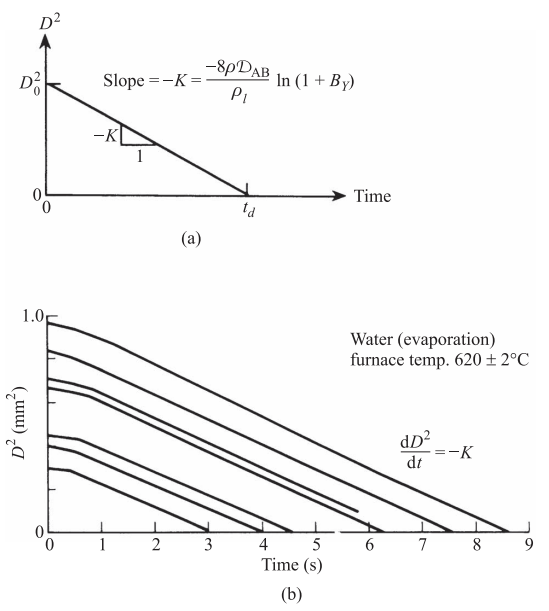
\includegraphics[width=.3\textwidth]{img/d2.png}
\end{figure}


\end{multicols}


\end{document}